\begin{center}
\textbf{\large Supplementary Material: \papertitle}
\end{center}

\section{Autoregressive evolution model} % (fold)
\label{sec:autoregressive_evolution_model}

\begin{itemize}
	\item Show the simplified expression for H=1
	\item discuss irreversibility, with example
\end{itemize}

% section autoregressive_evolution_model (end)

\section{Supplementary figures} % (fold)
\label{sec:supplementary_figures}

\begin{figure}[h]
	\centering
	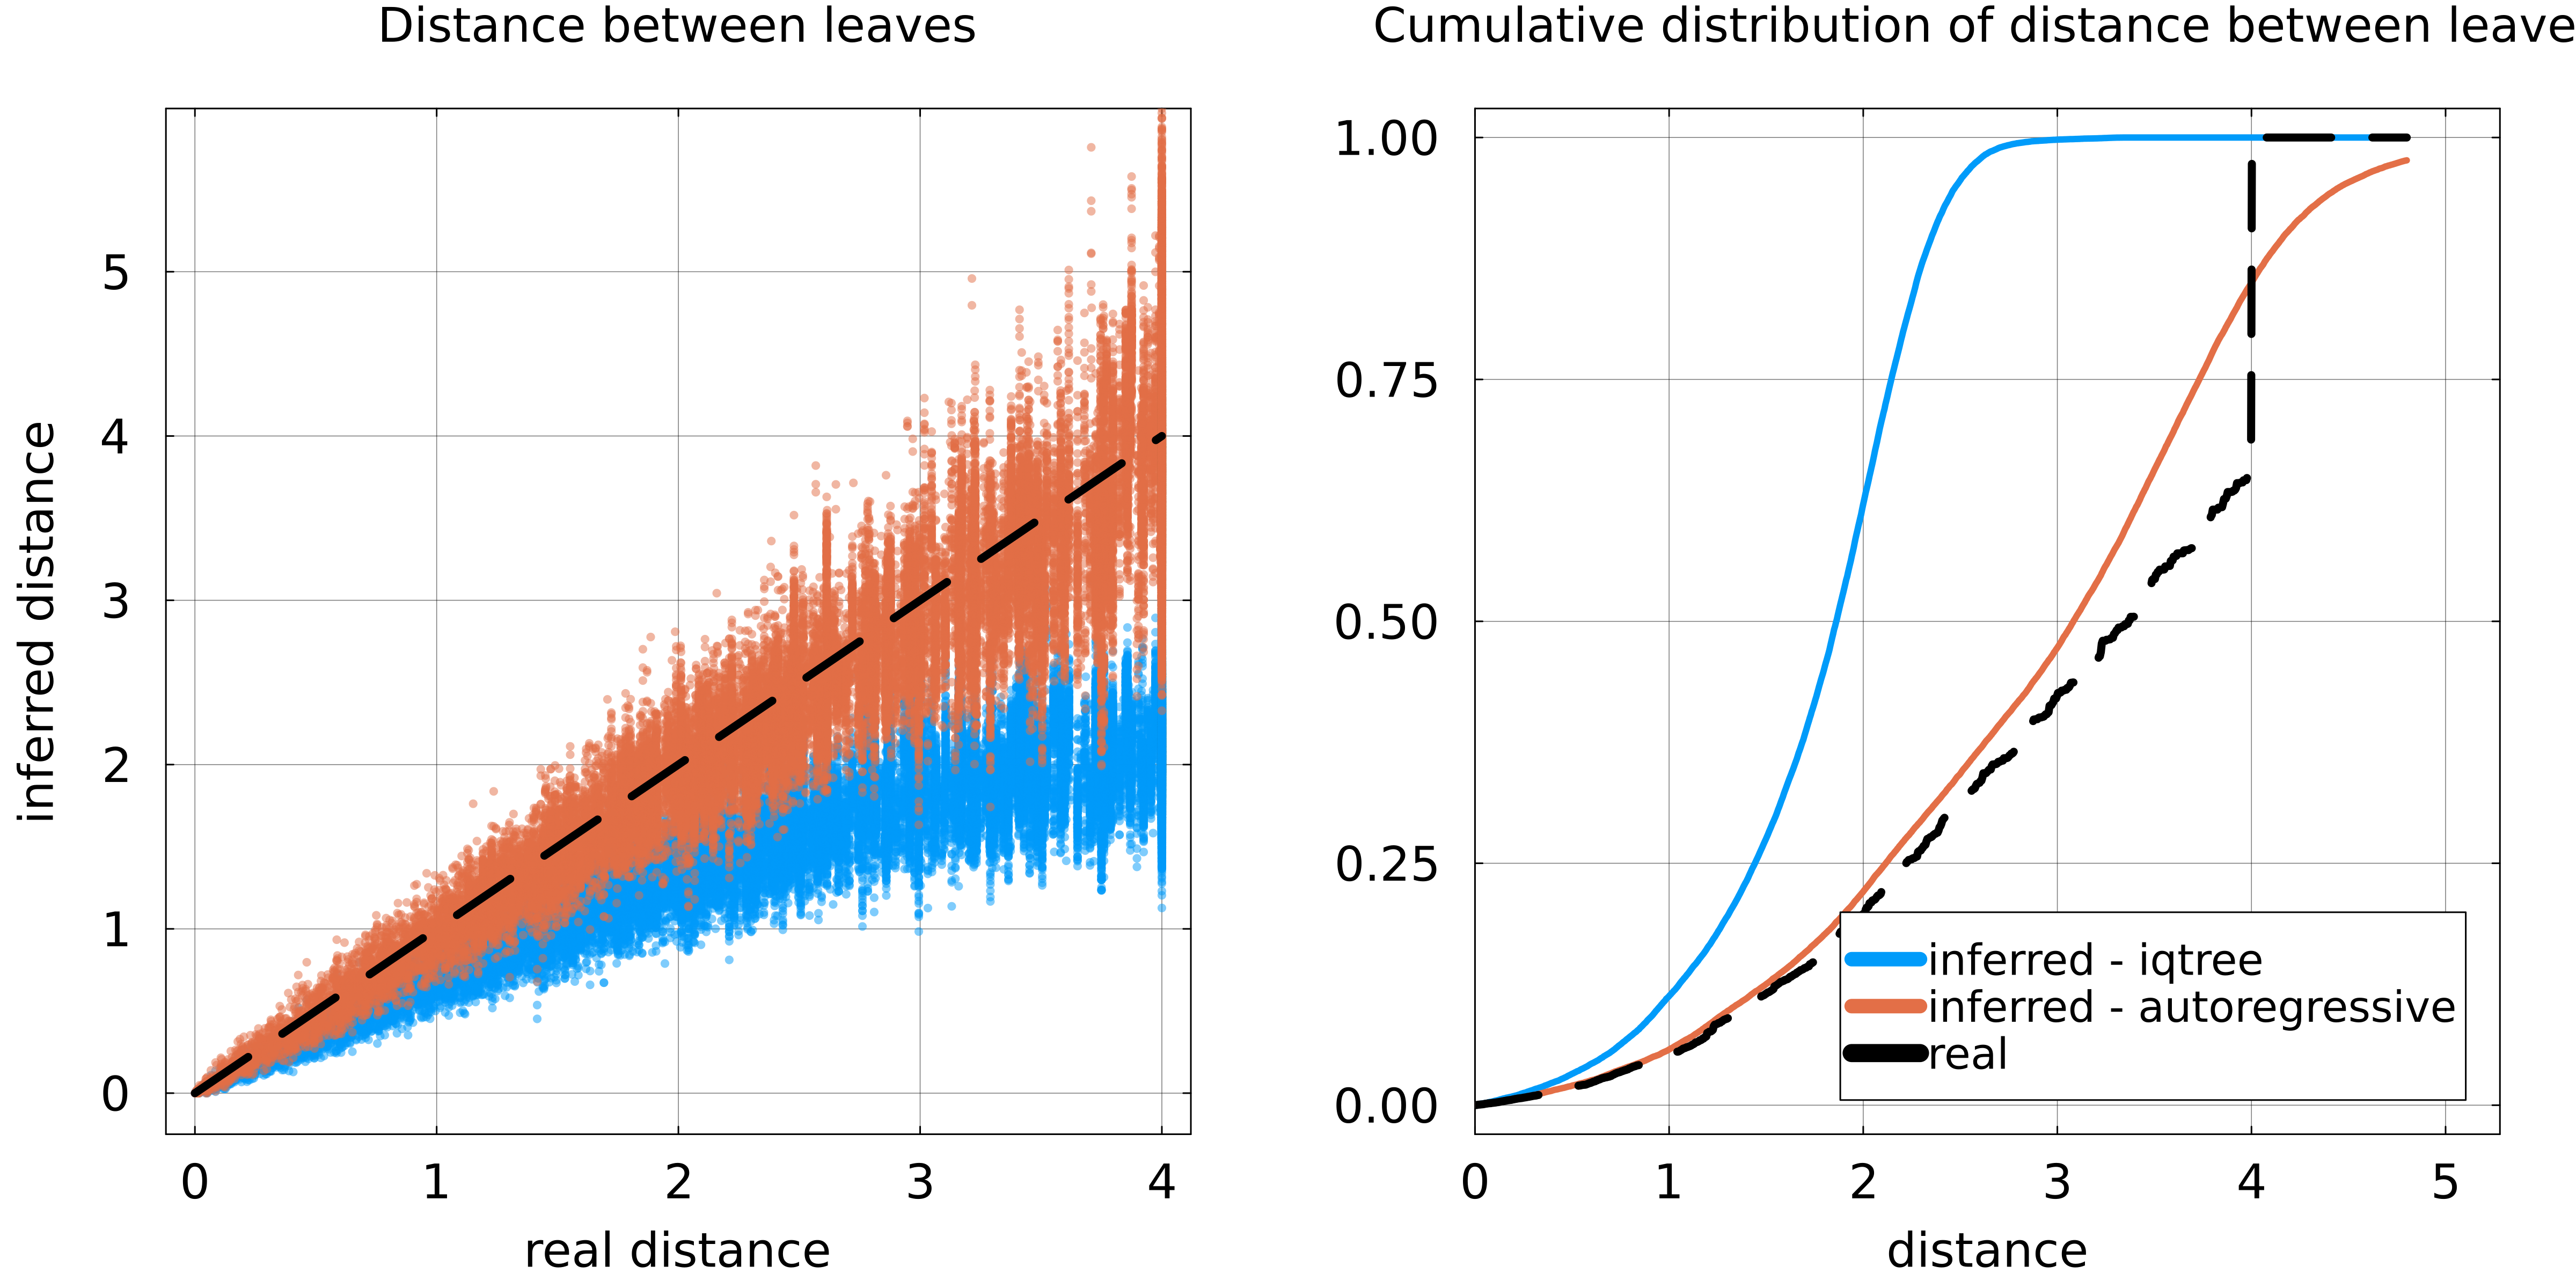
\includegraphics[width=.75\textwidth]{figures/SI/branch_length_reconstruction_arnet_PF00072.png}
	\caption{
		Quality of branch length inference using data simulated with the autoregressive evolver. 
		Inference is performed using the topology of a tree and leaf sequences generated using the autoregressive evolver. 
		Two techniques are compared: IQ-TREE and the profile model corresponding to the autoregressive evolver. 
		\textbf{Left}: inferred distance vs distance in the real trees for every pair of leaves. 
		\textbf{Right}: Cumulative distribution of pairwise distance between leaves for the two inference methods and for the real trees. 
		The discontinuity in the curve for the real tree is caused by the ultrametricity and fixed total height of the generated trees. 
	}
	\label{sfig:branch_length_reconstruction}
\end{figure}

\begin{figure}[h]
	\centering
	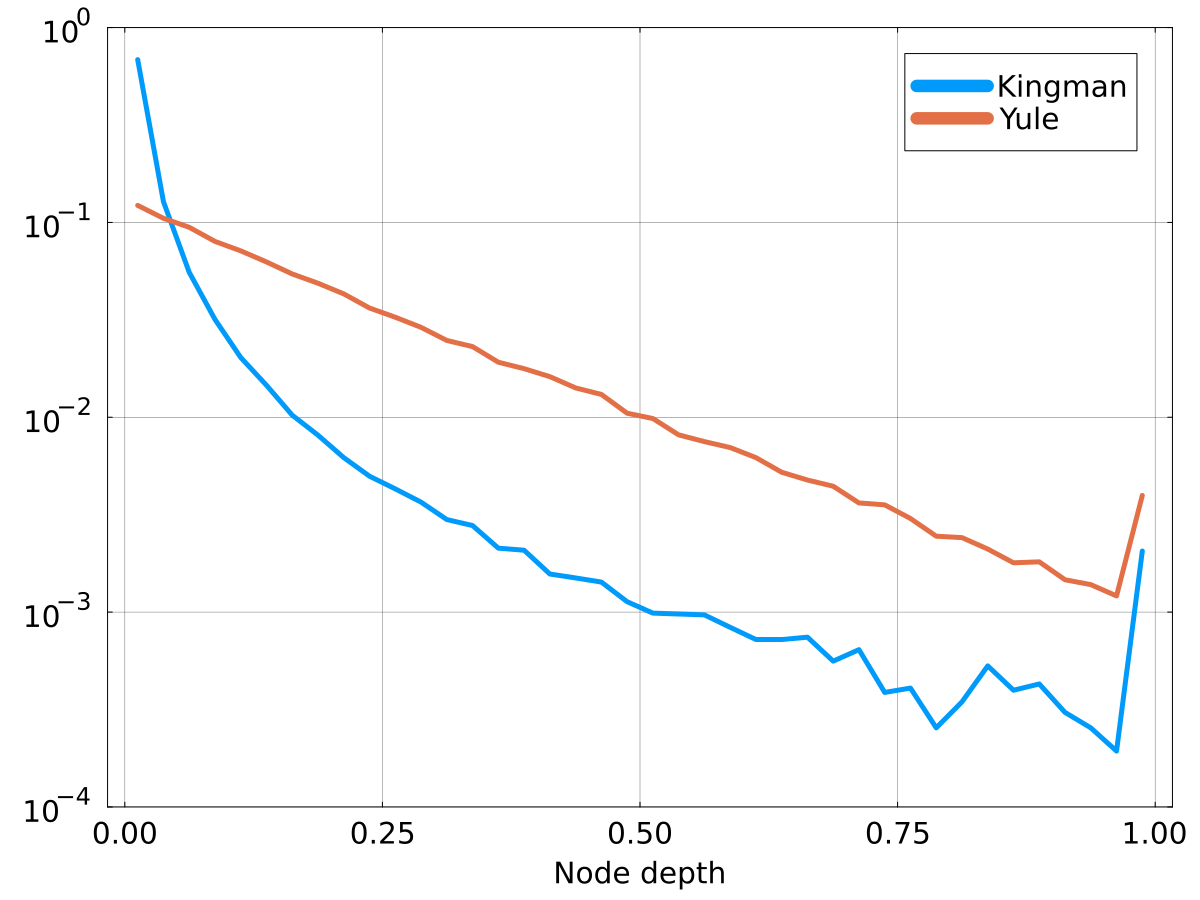
\includegraphics[width=.75\textwidth]{figures/SI/depth_distribution_coalescents.png}
	\caption{
		Distribution of node depth for trees coming from the Kingman and Yule coalescents. 
		Node depth is defined as the distance from a node to the closest leaf. 
		Data is obtained by sampling several trees from each coalescent. 
		Heights of trees are normalized to one. 
		The Kingman process concentrates most of the nodes in close vicinity to the leaves, while the Yule process spreads them more evenly. 
	}
	\label{sfig:depth_distribution_coalescent}
\end{figure}

% section supplementary_figures (end)